% !TeX root = ../main.tex
\documentclass[class=article]{standalone}

\begin{document}
\section*{Question 2}


\begin{center}
  \begin{tabular}{|rcl|rcl|}
      \hline
      \multicolumn{3}{|c}{\bf Productions} &
      \multicolumn{3}{|c|}{\bf Règles Sémantiques} \\
      \hline
      \hline
      $S$ & $\rightarrow$ & T & $T.hniv$ & $:=$ & $0$ \\
          &               &   & $T.hminv$ & $:=$ & $-\infty$\\
          &               &   & $T.hmaxv$ & $:=$ & $\infty$\\
          &               &   & $S.ok$ & $:=$ & $T.okv$ $\wedge$ $T.okn$\\
      \hline
      $T$ & $\rightarrow$ & \lstinline[]$[$ $T_1$ \lstinline[]$,$ {\bf num} \lstinline[]$,$ $T_2$ \lstinline[]$]$ & $T_1.hniv$ & $:=$ & $T.hniv + 1$ \\
          &               &                                                                                       & $T_2.hniv$ & $:=$ & $T.hniv + 1$\\
          &               &                                                                                       & $T_1.hminv$  & $:=$ & $T.hminv$\\
          &               &                                                                                       & $T_1.hmaxv$  & $:=$ & ${\bf num}.lexval$\\
          &               &                                                                                       & $T_2.hminv$  & $:=$ & ${\bf num}.lexval$\\
          &               &                                                                                       & $T_2.hmaxv$  & $:=$ & $T.hmaxv$\\
          &               &                                                                                       & $T.minv$  & $:=$ & $T_1.minv$\\
          &               &                                                                                       & $T.maxv$  & $:=$ & $T_2.maxv$\\
          &               &                                                                                       & $T.maxn$  & $:=$ & $T_1.maxn$\\
          &               &                                                                                       & $T.okv$   & $:=$ & $T_1.maxv \leq {\bf num}.lexval$\\
          &               &                                                                                       &           &      & $\wedge$ ${\bf num}.lexval \leq T_2.minv$\\
          &               &                                                                                       &           &      & $\wedge$ $T_1.okv$ $\wedge$ $T_2.okv$\\
          &               &                                                                                       & $T.okn$   & $:=$ & $T_1.maxn = T_2.maxn$\\
          &               &                                                                                       &           &      & $\wedge$ $T_1.okn$ $\wedge$ $T_2.okn$\\
      \hline
      \hline
      \multicolumn{6}{|c|}{[Voir page suivante]} \\
      \hline
  \end{tabular}
\end{center}

\begin{center}
  \begin{tabular}{|rcl|rcl|}
    \hline
    \multicolumn{6}{|c|}{[Voir page précédente]} \\
    \hline
    \hline
    $T$ & $\rightarrow$ & \lstinline[]$[$ $T_1$ \lstinline[]$,$ {\bf num$_1$} \lstinline[]$,$  $T_2$ \lstinline[]$,$ {\bf num$_2$} \lstinline[]$,$ $T_3$ \lstinline[]$]$  & $T_1.hniv$ & $:=$ & $T.hniv + 1$ \\
        &               &                                                                                                                                                 & $T_2.hniv$ & $:=$ & $T.hniv + 1$\\
        &               &                                                                                                                                                 & $T_3.hniv$ & $:=$ & $T.hniv + 1$\\
        &               &                                                                                                                                                 & $T_1.hminv$  & $:=$ & $T.hminv$\\
        &               &                                                                                                                                                 & $T_1.hmaxv$  & $:=$ & ${\bf num}_1.lexval$\\
        &               &                                                                                                                                                 & $T_2.hminv$  & $:=$ & ${\bf num}_1.lexval$\\
        &               &                                                                                                                                                 & $T_2.hmaxv$  & $:=$ & ${\bf num}_2.lexval$\\
        &               &                                                                                                                                                 & $T_3.hminv$  & $:=$ & ${\bf num}_2.lexval$\\
        &               &                                                                                                                                                 & $T_3.hmaxv$  & $:=$ & $T.hmaxv$\\
        &               &                                                                                                                                                 & $T.minv$  & $:=$ & $T_1.minv$\\
        &               &                                                                                                                                                 & $T.maxv$  & $:=$ & $T_3.maxv$\\
        &               &                                                                                                                                                 & $T.maxn$  & $:=$ & $T_1.maxn$\\
        &               &                                                                                                                                                 & $T.okv$   & $:=$ & $T_1.maxv \leq {\bf num}_1.lexval$\\
        &               &                                                                                                                                                 &           &      & $\wedge$ ${\bf num}_1.lexval \leq T_2.minv$\\
        &               &                                                                                                                                                 &           &      & $\wedge$ $T_2.maxv \leq {\bf num}_2.lexval$ \\
        &               &                                                                                                                                                 &           &      & $\wedge$ ${\bf num}_2.lexval \leq T_3.minv$\\
        &               &                                                                                                                                                 &           &      & $\wedge$ $T_1.okv$ $\wedge$ $T_2.okv$\\
        &               &                                                                                                                                                 &           &      & $\wedge$ $T_3.okv$\\
        &               &                                                                                                                                                 & $T.okn$   & $:=$ & $T_1.maxn = T_2.maxn$\\
        &               &                                                                                                                                                 &           &      & $\wedge$ $T_2.maxn = T_3.maxn$\\
        &               &                                                                                                                                                 &           &      & $\wedge$ $T_1.okn$ $\wedge$ $T_2.okn$\\
        &               &                                                                                                                                                 &           &      & $\wedge$ $T_3.okn$\\
    \hline
    $T$ & $\rightarrow$ & \lstinline[]$[]$  & $T.minv$ & $:=$ & $T.hminv$\\
        &               &                   & $T.maxv$ & $:=$ & $T.hmaxv$\\
        &               &                   & $T.maxn$ & $:=$ & $T.hniv$\\
        &               &                   & $T.okv$ & $:=$ & $T.minv \leq T.maxv$\\
        &               &                   & $T.okn$ & $:=$ & \lstinline[]$true$\\
    \hline
  \end{tabular}
\end{center}
\begin{center}
  \begin{tikzpicture}
    [
    sibling distance=2em, level distance=30pt]

    \tikzset{edge from parent/.style={,draw, edge from parent path=
    {(\tikzparentnode) -- (\tikzchildnode)}}}
    \Tree 
    [.$S\tbox{ok}{true}\tbox{gen}{""}\tbox{cod}{""}$ 
      [.$\tbox{hniv}{0}\tbox{hminv}{-inf}\tbox{hmaxv}{inf}T\tbox{minv}{-infinity}\tbox{maxv}{12}\tbox{maxn}{}\tbox{okv}{}\tbox{okn}{}$
        [.$\tbox{hniv}{1}\tbox{hminv}{-inf}\tbox{hmaxv}{12}T\tbox{minv}{-inf}\tbox{maxv}{12}\tbox{maxn}{2}\tbox{okv}{}\tbox{okn}{}$
          [.$\tbox{hniv}{2}\tbox{hminv}{-inf}\tbox{hmaxv}{14}T\tbox{minv}{-inf}\tbox{maxv}{14}\tbox{maxn}{2}\tbox{okv}{true}\tbox{okn}{true}$
            $[]$
          ]
          14
          [.$\tbox{hniv}{2}\tbox{hminv}{14}\tbox{hmaxv}{12}T\tbox{minv}{14}\tbox{maxv}{12}\tbox{maxn}{2}\tbox{okv}{true}\tbox{okn}{true}$
            $[]$
          ]
        ]
      ]
    ]
  \end{tikzpicture}
\end{center}

\end{document}